%\chapter{\normalsize{BACKGROUND OF SATELLITE REMOTE SENSING}}
\chapter{\normalsize{RESULTS}}
\paragraph{}
This chapter deals about the outcome of our analysis and how to share the results with the community.
%\section{Technique 5: Processing satellite data using GIS Software}
\section{Extract chart command line tools.}
\subsection{Visualise temperature chart.}
\begin{lstlisting}[language=Bash]
# Visualize data
#Set date and time on 31 January 2021 at 03:00 UTC
dt="20210131.0300"
#Set date and time on 31 January 2021 at 03:00 UTC
#dt="20210131.1500"
# Open a monitor
d.mon wx0
#set the coordinate grid
d.grid 3
# Display a raster map
d.rast GLDAS_NOAH025_3H_A${dt}_Tair_final
# Display a vector map
d.vect map=cmr type=boundary
#Add text
#d.text text="31 JAN 2021 0300Z" color=black bgcolor=white size=3
d.text text="31 JAN 2021 1500Z" color=black bgcolor=white size=3
# Add raster legend
# Add raster legend
d.legend -t -s -b raster=GLDAS_NOAH025_3H_A${dt}_Tair_final title=TEMPERATURE title_fontsize=20 font=sans fontsize=18
# Add North arrow
d.northarrow style=1b text_color=black
# press enter
\end{lstlisting}
\begin{figure}[H]
\begin{center}
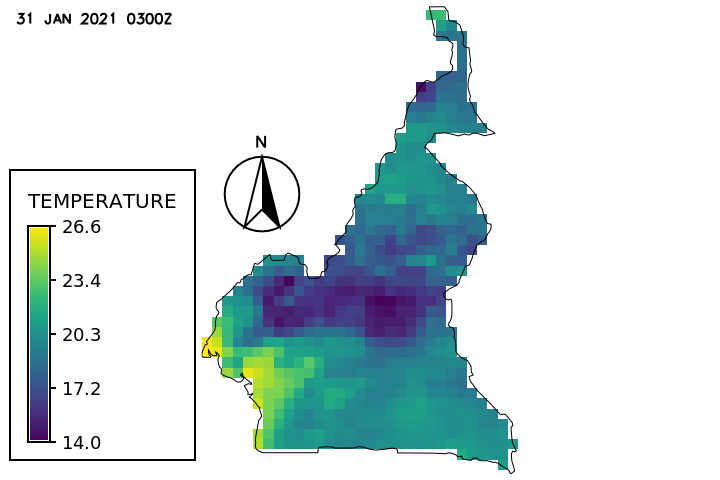
\includegraphics[scale=0.6]{tp03.png} %\cite{umhe}
\end{center}

\caption{Temperature at 03:00 UTC}
\label{Temperature at 03:00 UTC}%\cite{ABIA}
\end{figure}
\begin{figure}[H]
\begin{center}
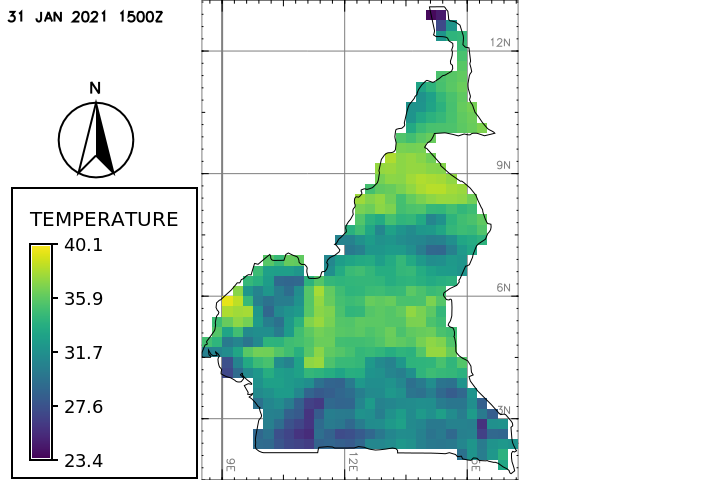
\includegraphics[scale=0.6]{tp15a.png} %\cite{umhe}
\end{center}
\caption{Temperature at 15:00 UTC}
\label{Temperature at 15:00 UTC}%\cite{ABIA}
\end{figure}

\section{Relative Humidity Chart}
\begin{lstlisting}[language=Bash]
dt="20210131.0300"
#dt="20210131.1500"
# Visualize data
r.mask vect=cmr --o
# Open a monitor
d.mon wx0
# Display a raster map
d.rast GLDAS_NOAH025_3H_A${dt}_Rh_final
# Display a vector map
d.vect map=cmr type=boundary
d.text text="31 JAN 2021 0300Z" color=black bgcolor=white size=3
# Add raster legend
d.legend -t -s -b raster=GLDAS_NOAH025_3H_A${dt}_Rh_final title=RELATIVE HUMIDITY title_fontsize=20 font=sans fontsize=18
# Add North arrow
d.northarrow style=1b text_color=black
#Clear the monitor
#d.erase -f
#r.mask -r
\end{lstlisting}

\begin{figure}[H]
\begin{center}
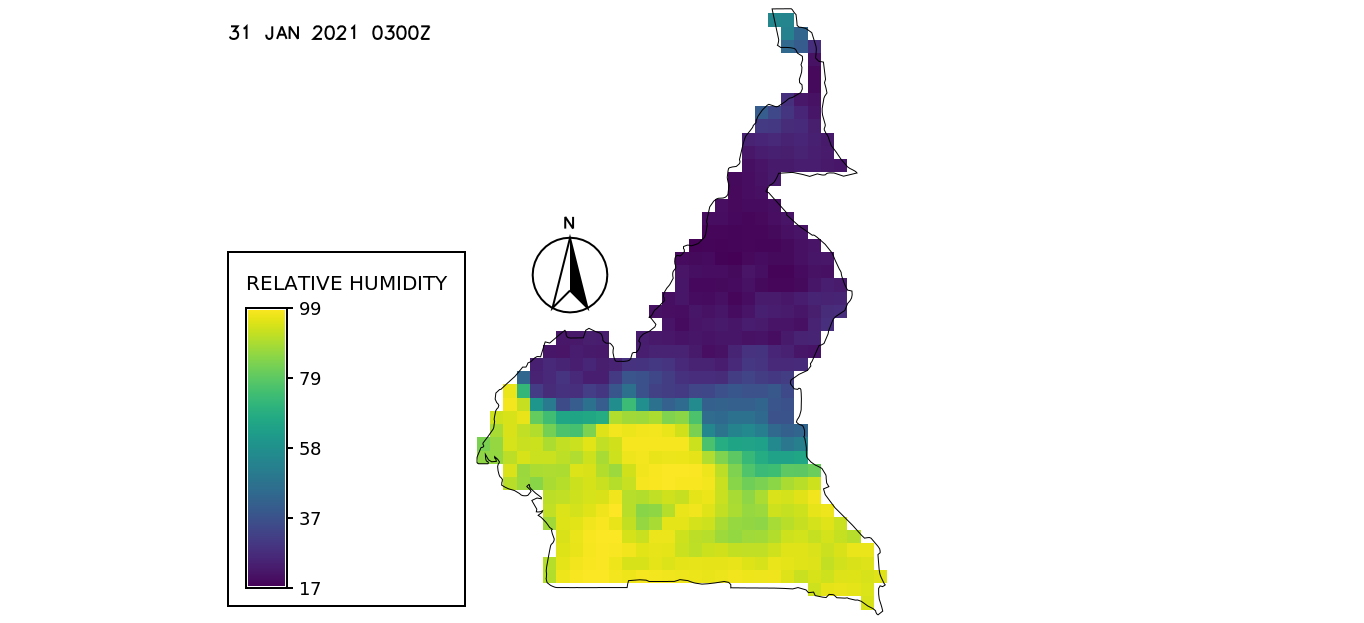
\includegraphics[scale=0.6]{rh03.png} %\cite{umhe}
\end{center}
\caption{Relative Humidity at 03:00 UTC}
\label{Relative Humidity at 03:00 UTC}%\cite{ABIA}
\end{figure}

\begin{figure}[H]
\begin{center}
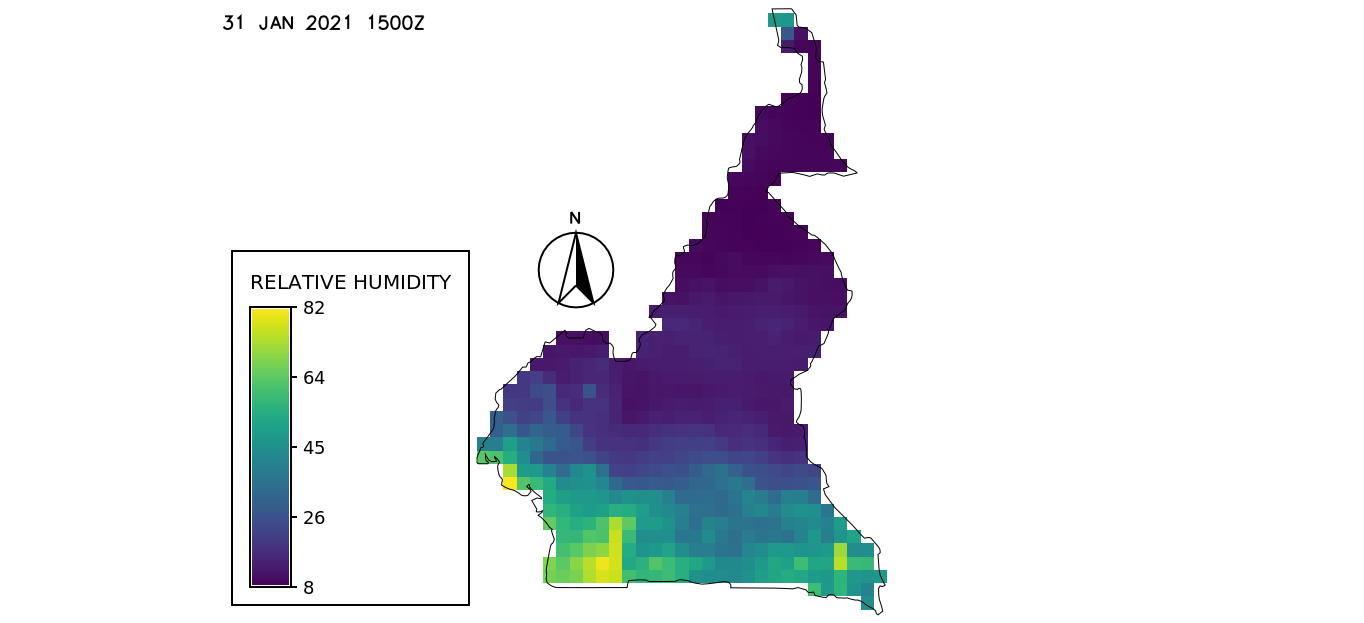
\includegraphics[scale=0.6]{rh15.png} %\cite{umhe}
\end{center}
\caption{Relative Humidity at 15:00 UTC}
\label{Relative Humidity at 15:00 UTC}%\cite{ABIA}
\end{figure}

\section{Surface Pressure Chart}
\begin{lstlisting}[language=Bash]
#dt="20210131.0300"
dt="20210131.1500"
# Visualize data
r.mask vect=cmr --o
# Open a monitor
d.mon wx0
# Display a raster map
d.rast GLDAS_NOAH025_3H_A${dt}_Psurf_final 
# Display a vector map
d.vect map=cmr type=boundary
d.text text="31 JAN 2021 1500Z" color=black bgcolor=white size=3
# Add raster legend
d.legend -t -s -b raster=GLDAS_NOAH025_3H_A${dt}_Psurf_final title="SURFACE PRESSURE (Pa)" title_fontsize=20 font=sans fontsize=18
# Add North arrow
d.northarrow style=1b text_color=black
#d.erase -f
#r.mask -r
\end{lstlisting}

\begin{figure}[H]
\begin{center}
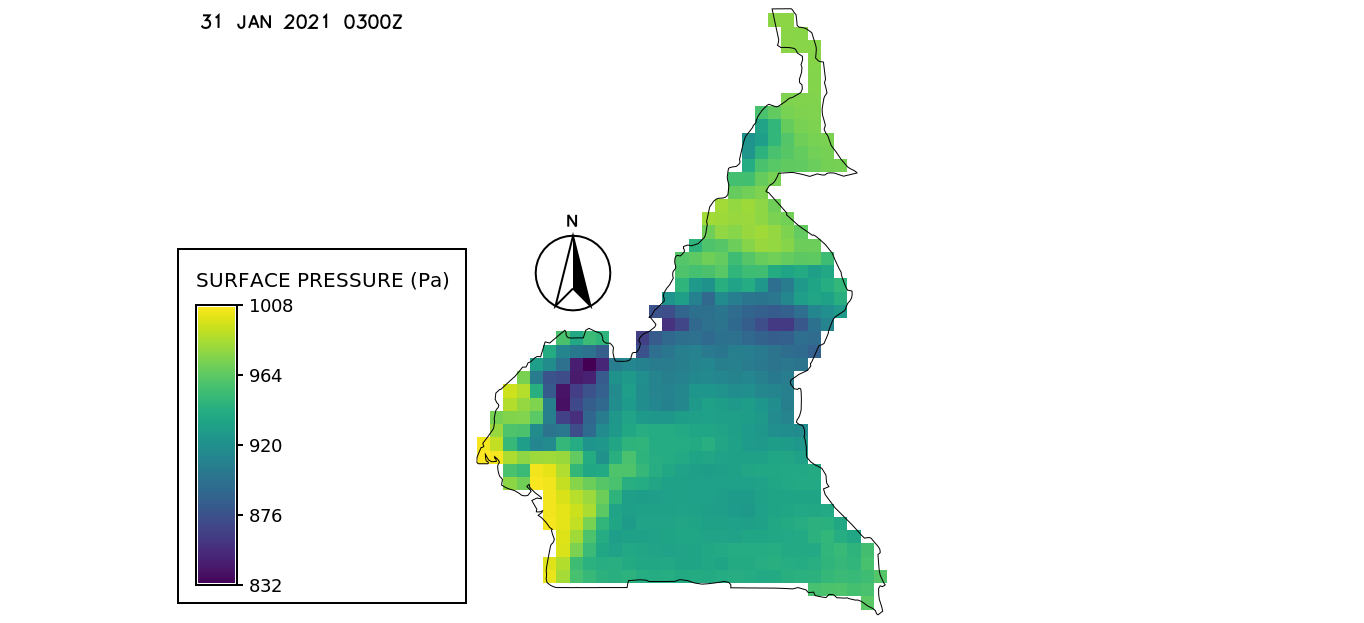
\includegraphics[scale=0.6]{sp03.png} %\cite{umhe}
\end{center}
\caption{Surface Pressure at 03:00 UTC}
\label{Surface Pressure  at 03:00 UTC}%\cite{ABIA}
\end{figure}

\begin{figure}[H]
\begin{center}
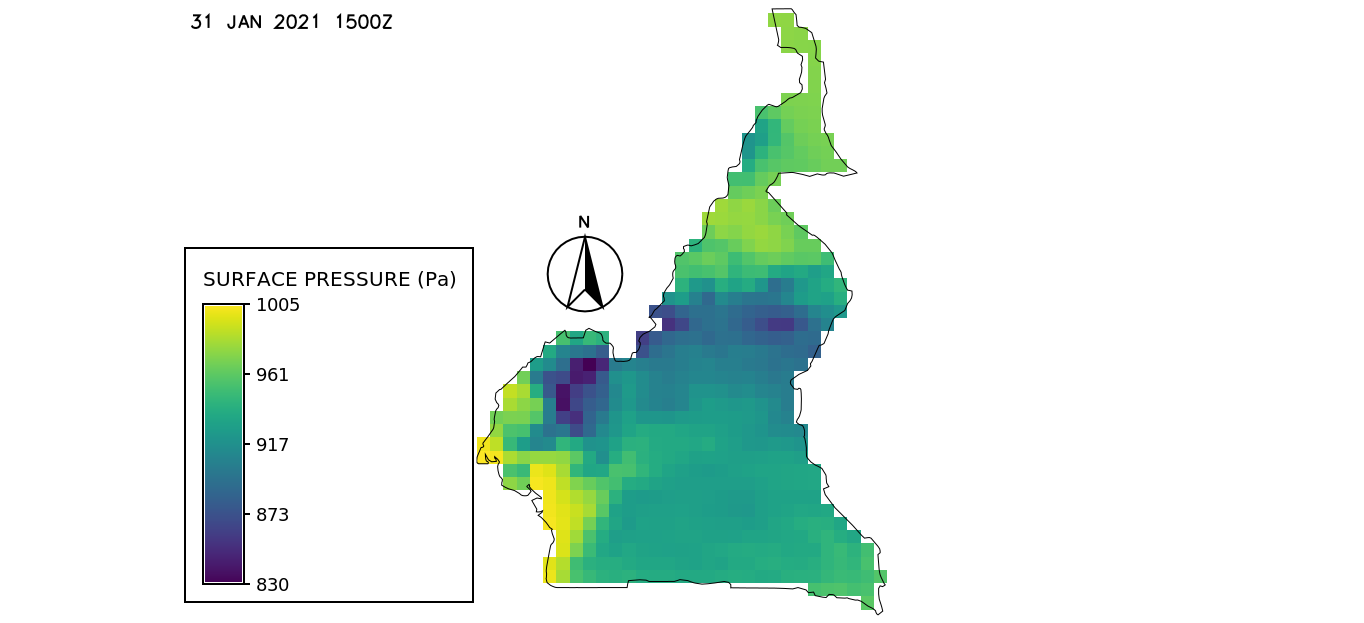
\includegraphics[scale=0.6]{sp15.png} %\cite{umhe}
\end{center}
\caption{Surface Pressure  at 15:00 UTC}
\label{Surface Pressure  at 15:00 UTC}%\cite{ABIA}
\end{figure}


\section{Wind Speed Chart}
\begin{lstlisting}[language=Bash]
#dt="20210131.0300"
dt="20210131.1500"
# Visualize data
r.mask vect=cmr --o
# Open a monitor
d.mon wx0
# Display a raster map
d.rast GLDAS_NOAH025_3H_A${dt}_Wind_final
# Display a vector map
d.vect map=cmr type=boundary
d.text text="31 JAN 2021 1500Z" color=black bgcolor=white size=3
# Add raster legend
d.legend -t -s -b raster=GLDAS_NOAH025_3H_A${dt}_Wind_final title="WIND SPEED m/s" title_fontsize=20 font=sans fontsize=18
#Add North arrowd.northarrow style=1b text_color=black
d.northarrow style=1b text_color=black
#d.erase -f
#r.mask -r

\end{lstlisting}

\begin{figure}[H]
\begin{center}
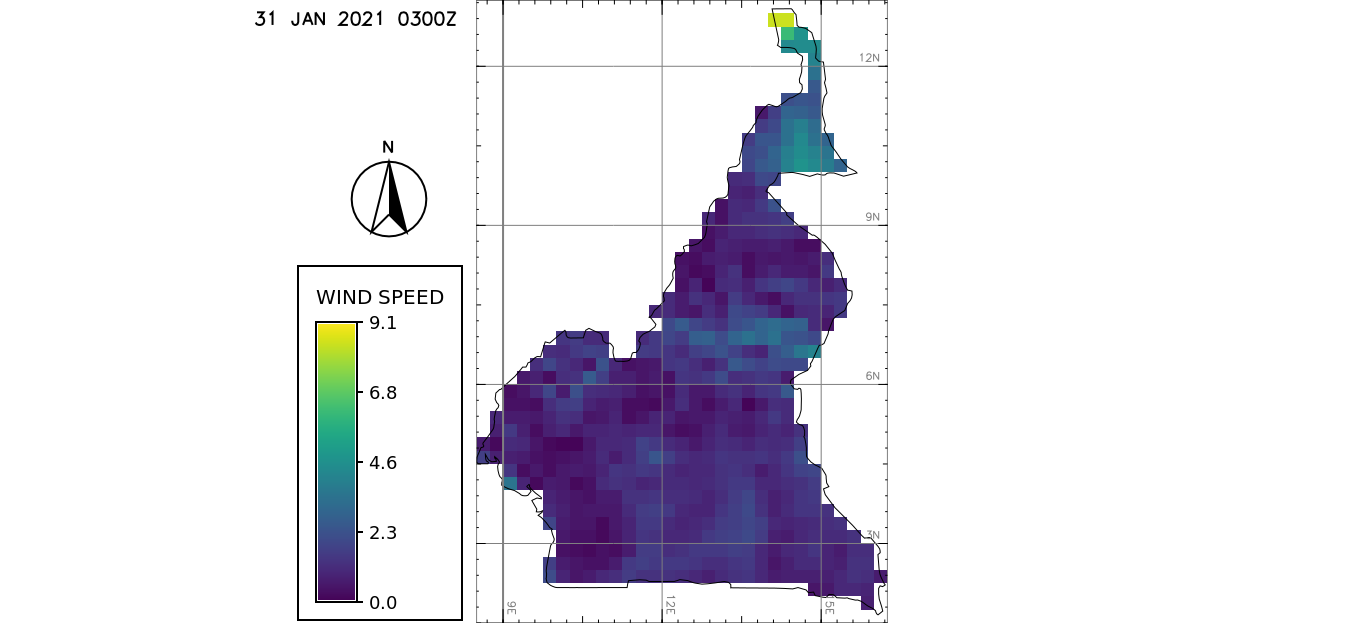
\includegraphics[scale=0.6]{ws03.png} %\cite{umhe}
\end{center}
\caption{Wind Speed at 03:00 UTC}
\label{Surface Pressure  at 03:00 UTC}%\cite{ABIA}
\end{figure}

\begin{figure}[H]
\begin{center}
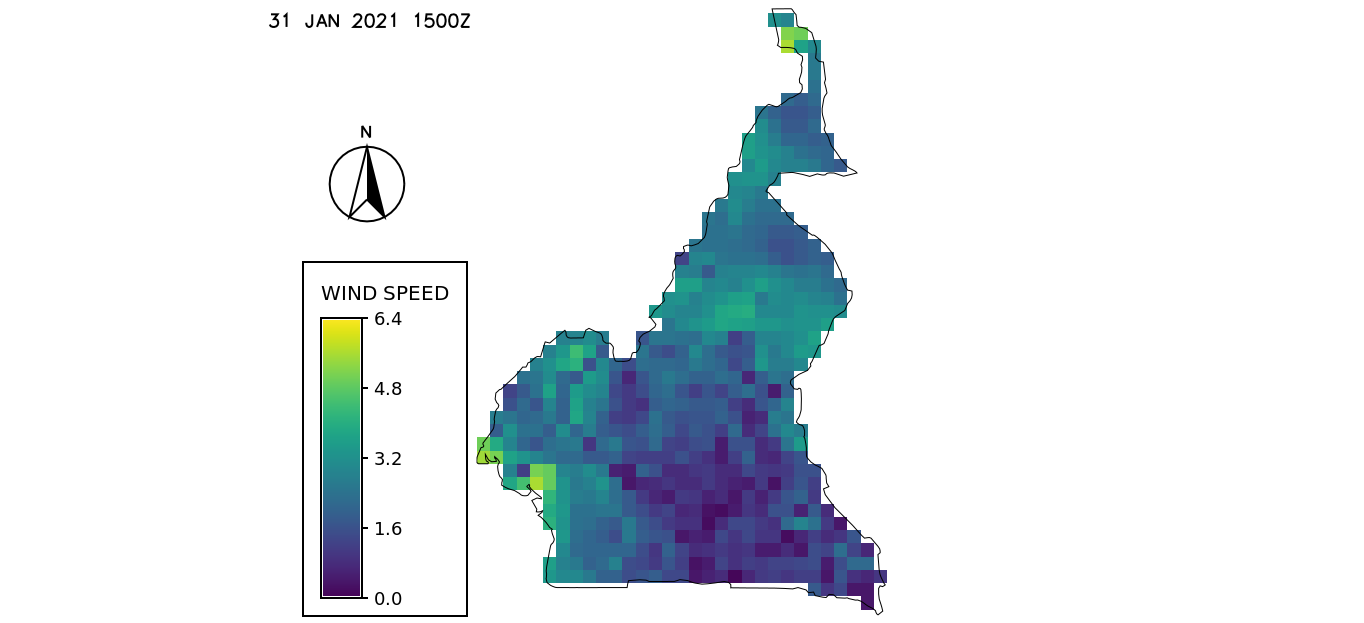
\includegraphics[scale=0.6]{ws15.png} %\cite{umhe}
\end{center}
\caption{Wind Speed at 15:00 UTC}
\label{Surface Pressure  at 15:00 UTC}%\cite{ABIA}
\end{figure}


  \begin{table}[H]
\caption{Tableau comparatif des technologies biométriques}
\label{Tableau comparatif des technologies biométriques} \cite{cabs}
\begin{center}
\begin{tabular}{|c|c|c|c|c|c|c|c|}
\hline
\multirow{2}*{ \textbf{Biométrie}} & \multicolumn{7}{c|}{\textbf{Exigences}}\\
\cline{2-8}
  & \rotatebox {45}{Universalité\,} & \rotatebox {45}{Unicité\,}& \rotatebox {45}{Permanence\,} & \rotatebox {45}{Collectabilité\,} & \rotatebox {45}{Performance\,} & \rotatebox {45}{Acceptabilité\,}& \rotatebox {45}{Sécurité\,}  \\ \hline
 Face& E & F  & M & E & F  & E & E   \\[2pt] \hline
 Main & M & M & M & E  & M & M & M   \\[2pt] \hline
 \textcolor{magenta} {Empreinte} &\textcolor{magenta} { M} &\textcolor{magenta} {E} &\textcolor{magenta} {E } &\textcolor{magenta} { M } & \textcolor{magenta} { E} & \textcolor{magenta} { M} &  \textcolor{magenta} {M }  \\[2pt] \hline
 Iris  & E & E  & E & M & E & F & F \\[2pt] \hline
 Rétine & E & E & M & F & E & F & F   \\[2pt] \hline
  keystroke & F & F & F & M & F & M & M  \\[2pt] \hline
  Voix & M & F & F & M & F  & E & E \\[2pt] \hline
  Signature & F & F & F & E & F & E & E  \\[2pt] \hline
  
 \end{tabular}
\end{center}
\end{table}


 \begin{table}[H]
\caption{Tableau comparatif des technologies biométriques}
\label{Tableau comparatif des technologies biométriques} \cite{cabs}
\begin{center}
\begin{tabular}{|c|c|c|c|c|c|c|c|c|c|c|c|c|}
\hline
\multirow{2}*{ \textbf{Time (UTC)}} & \multicolumn{12}{c|}{\textbf{Bafoussam aviation meteorological station}}\\
\cline{2-13}
  & \rotatebox {45}{Tair1\,} & \rotatebox {45}{Tair2\,}& \rotatebox {45}{DTair\,} & \rotatebox {45}{Rh1\,} & \rotatebox {45}{Rh2\,} & \rotatebox {45}{DRh\,}& \rotatebox {45}{Ws1\,} & \rotatebox {45}{Ws2\,}& \rotatebox {45}{DWs\,}& \rotatebox {45}{Ws2\,} &\rotatebox {45}{Ws2\,}&\rotatebox {45}{Ws2\,} \\ \hline
 00:00& E & F  & M & E & F  & E & E  & E& E& E& E & E  \\[2pt] \hline
03:00 & M & M & M & E  & M & M & M  & E & E& E& E & E \\[2pt] \hline
 \textcolor{magenta} {06:00} &\textcolor{magenta} { M} &\textcolor{magenta} {E} &\textcolor{magenta} {E } &\textcolor{magenta} { M } & \textcolor{magenta} { E} & \textcolor{magenta} { M} &  \textcolor{magenta} {M } & E & E& E& E& E  \\[2pt] \hline
09:00  & E & E  & E & M & E & F & F & E& E& E& E& E  \\[2pt] \hline
12:00 & E & E & M & F & E & F & F  & E & E& E& E & E \\[2pt] \hline
15:00 & F & F & F & M & F & M & M & E  & E& E& E& E \\[2pt] \hline
  18:00 & M & F & F & M & F  & E & E & E & E& E& E& E \\[2pt] \hline
  21:00 & F & F & F & E & F & E & E & E  & E& E& E& E \\[2pt] \hline
  
 \end{tabular}
\end{center}
\end{table}[H]